\documentclass[a4paper]{scrartcl}

%% Language and font encodings
\usepackage[english]{babel}
\usepackage[utf8x]{inputenc}
\usepackage[T1]{fontenc}

%% Sets page size and margins
\usepackage[a4paper,top=3cm,bottom=2cm,left=3cm,right=3cm,marginparwidth=1.75cm]{geometry}

%% Useful packages
\usepackage{amsmath}
\usepackage{graphicx}
\usepackage{subcaption}
\usepackage[colorinlistoftodos]{todonotes}
\usepackage[colorlinks=true, allcolors=blue]{hyperref}
\usepackage{placeins}
\usepackage{siunitx}
\usepackage{sidecap}
\usepackage{float}
\DeclareSIUnit\atmosphere{atm}

\title{Computational Motor Control - Lab 4}
\author{Florian Kaufmann \and Octave Martin \and Matthias Tsai}

\begin{document}
\maketitle

\section{Introduction}
The aim of this laboratory is to model central pattern generators to simulate a primitive behaviour of a lamprey neural system. By varying the parameters, we are going to experiment different simulations to help us understand the weight of each parameter and how to modify the behaviour of our lamprey model.

\section{Modelling the lamprey CPG with phase oscillators}
\subsection{Default parameters (6a.)}

We implemented a different chains of oscillators and varied the number of oscillators, the gradient of frequencies between them as well the coupling strength. To start of, we chose 10 oscillators, a frequency gradient of $\pi /6$ and a coupling strength of 7 to get an example of a phase locked chain of oscillators (see \cite{6astable}). From the plots, one can observe that the phase differences between the oscillators all stabilize to constant values and the oscillators visibly synchronize (left plot). Furthermore, despite of the intrinsic frequency gradient, the oscillators all agree on a common frequency during the simulation (right plot).

\begin{figure}[!h]
	\centering
	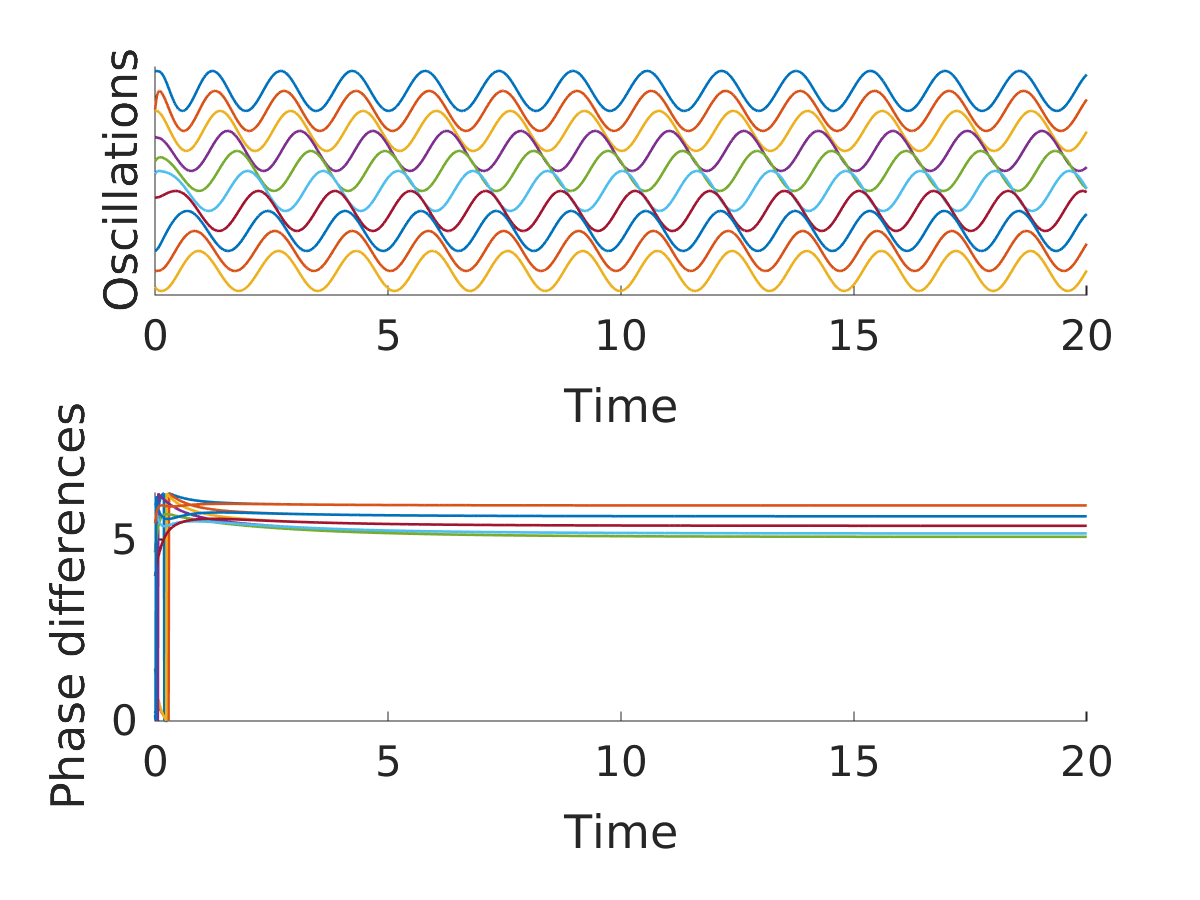
\includegraphics[width=0.5\textwidth]{fig/chain_phase_oscil-6a_stable.png}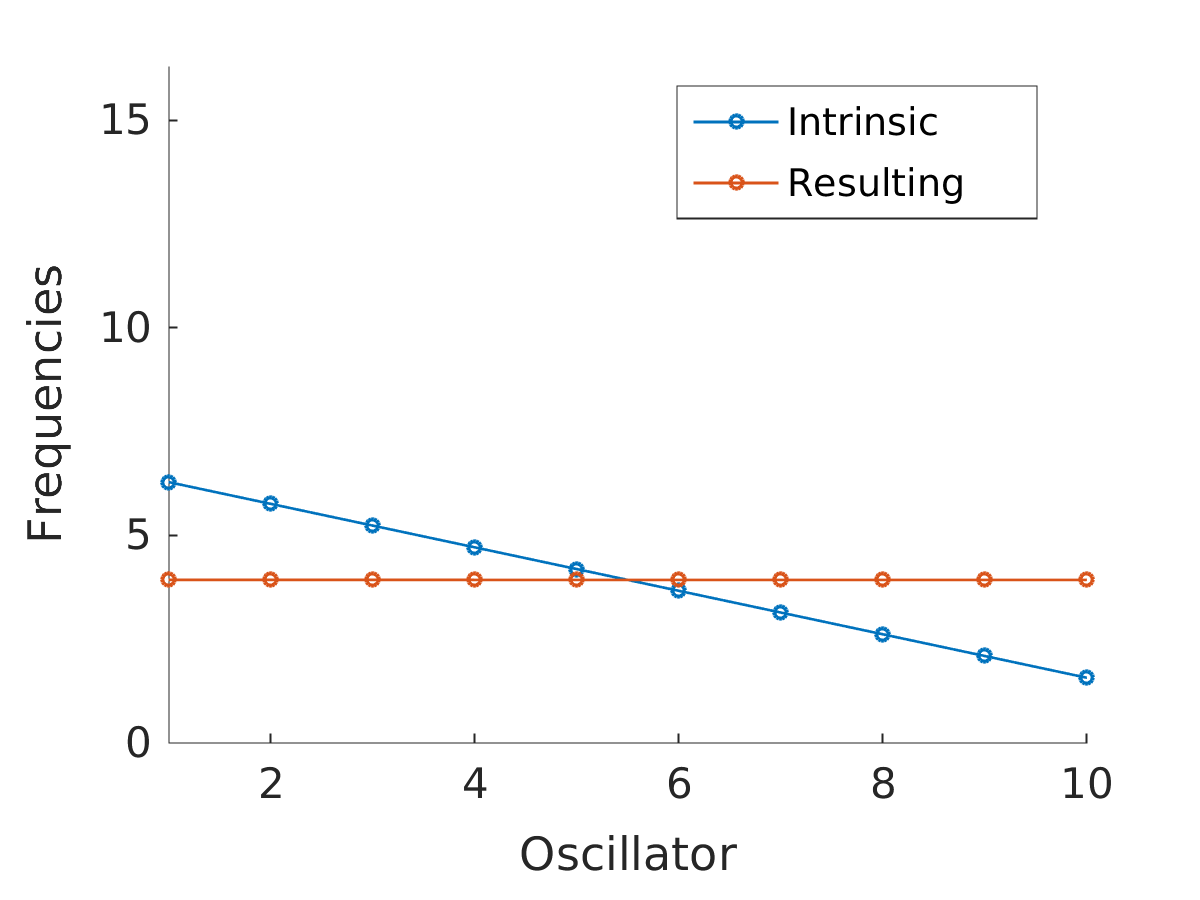
\includegraphics[width=0.5\textwidth]{fig/chain_phase_oscil_freq-6a_stable.png}
	\caption{Simulation of a chain of 10 phase oscillators with frequency gradient of $\pi /6$ and coupling strength of 7. Left: Oscillations and Phase differences of the oscillators over time.  Right: Plot of intrinsic frequencies and resulting frequencies from the simulation.}
\end{figure}

Next, we used our analytical formula to modify one parameter at a time to lose the phase locking behaviour of the chain of oscillators. First, the coupling strength was modified and reduced to 4 (see \cite{6aunstablecoupling}), and as predicted by our analytical prediction, the phase locking was lost. Interestingly, the chain of oscillators seems to have converged on two distinct frequencies, with the upper half of the chain synchronizing on a higher frequency as the lower part of the chain, with the central oscillators (especially the green one) experiencing quite some perturbation by being localized at the interface between these two subsystems.

\begin{figure}[!h]
	\centering
	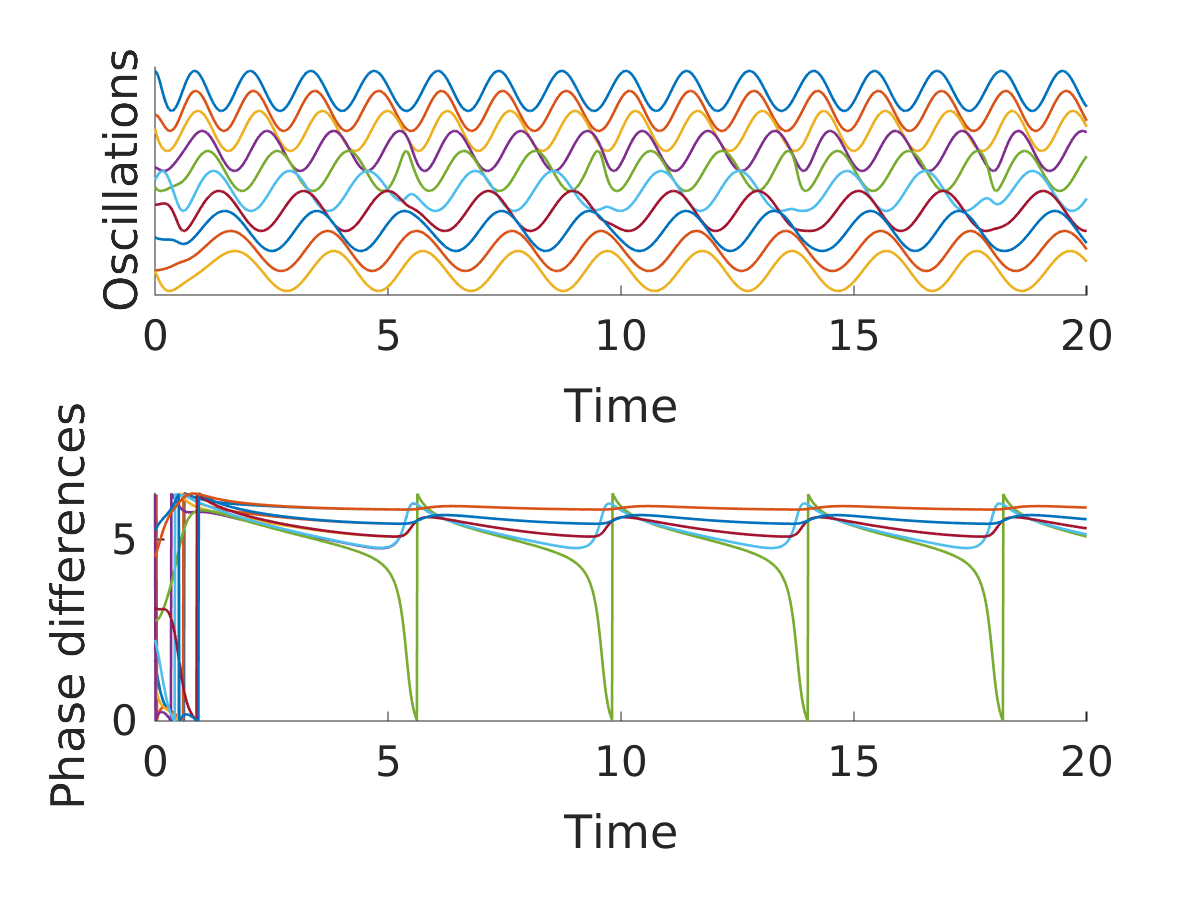
\includegraphics[width=0.5\textwidth]{fig/chain_phase_oscil-6a_unstable.png}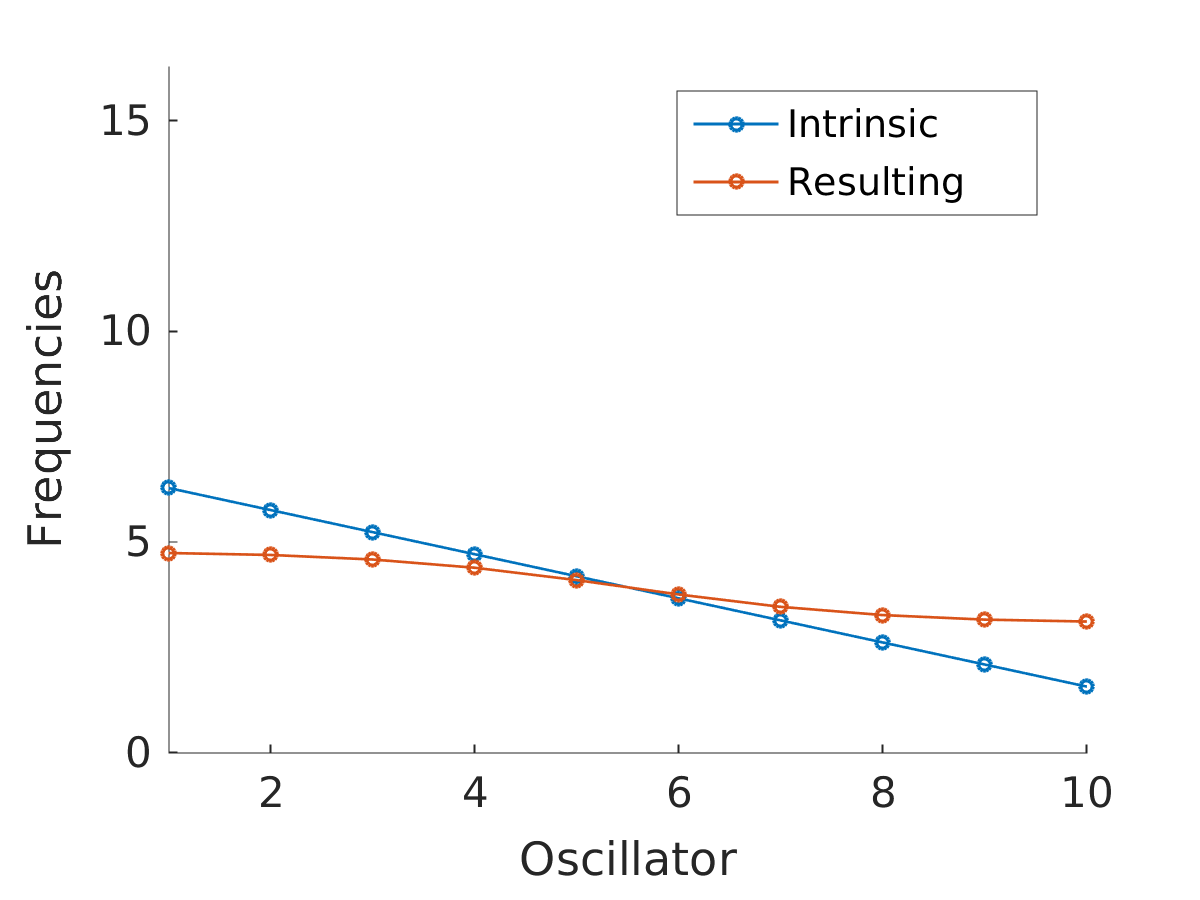
\includegraphics[width=0.5\textwidth]{fig/chain_phase_oscil_freq-6a_unstable.png}
	\caption{Simulation of a chain of 10 phase oscillators with frequency gradient of $\pi /6$ and coupling strength of 4. Left: Oscillations and Phase differences of the oscillators over time. Right: Plot of intrinsic frequencies and resulting frequencies from the simulation.}
\end{figure}

Similar loss of phase locking was also observed, if our initial phase locked oscillator chain was modified to either raise the frequency gradient to $\pi /5$ or to raise the number of oscillators to 11. This isn't very surprising, because by looking at the phase locking inequality condition using the parameters of our synchronized oscillator chain, one can predict that already a small change of one parameter in the wrong direction would change the sign of the inequality.

\begin{equation}
	coupling \_ strength = 7 > 6.545 =\frac{\pi \cdot 10^{2}}{6 \cdot 8} = \frac{frequency \_ gradient \cdot Noscils^2}{8}
\end{equation}


\newpage


\begin{minipage}{0.33\textwidth}
	\begin{figure}[H]
		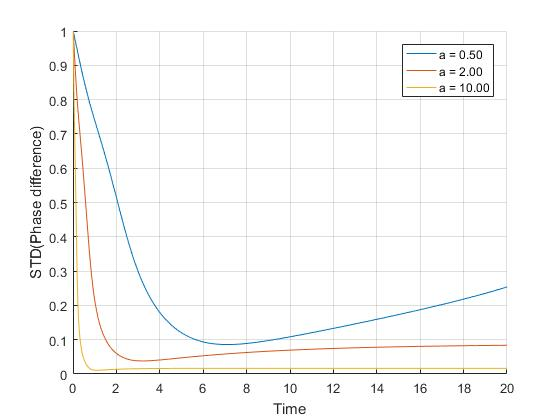
\includegraphics[width=\textwidth]{results/6.a/N10_E_const.jpg}
	\end{figure}
\end{minipage} \hfill
\begin{minipage}{0.33\textwidth}
	\begin{figure}[H]
		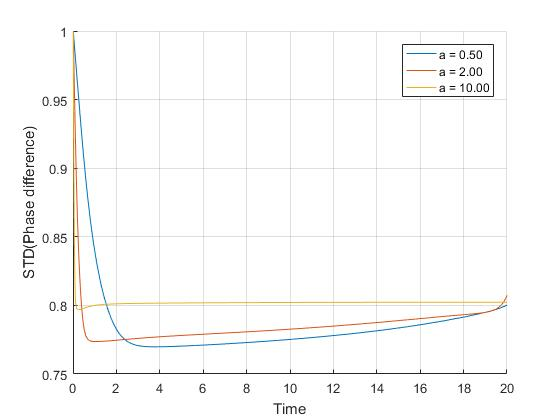
\includegraphics[width=\textwidth]{results/6.a/N20_E_const.jpg}
	\end{figure}
\end{minipage}\hfill
\begin{minipage}{0.33\textwidth}
	\begin{figure}[H]
		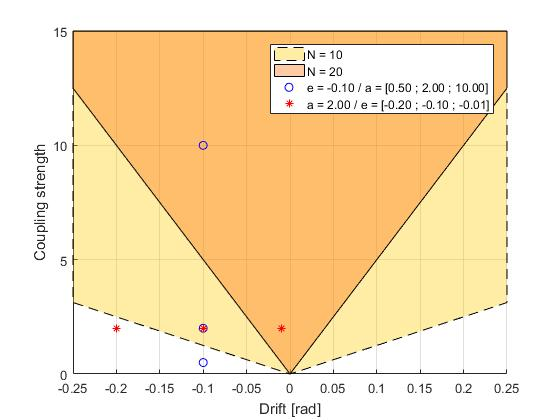
\includegraphics[width=\textwidth]{results/6.a/ArnoldTongue.jpg}
	\end{figure}
\end{minipage}
\begin{minipage}{0.33\textwidth}
	\begin{figure}[H]
		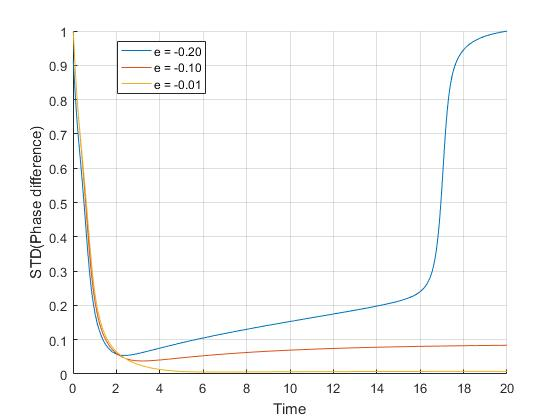
\includegraphics[width=\textwidth]{results/6.a/N10_A_const.jpg}
	\end{figure}
\end{minipage}
\begin{minipage}{0.33\textwidth}
	\begin{figure}[H]
		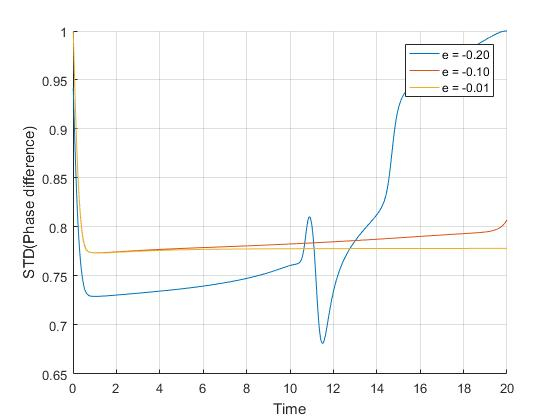
\includegraphics[width=\textwidth]{results/6.a/N20_A_const.jpg}
	\end{figure}
\end{minipage}\hfill
\begin{minipage}{0.33\textwidth}
	%just to align the figures
\end{minipage}

To check for phase locking regime, we look for stable phase differences between oscillators after a certain time of simulation. The standard deviation measures the spread of the variables, therefore the standard deviation of the phase differences between oscillators is constant in phase locking regime. 

The first four figures represent the standard deviation of the phase differences between oscillators as a function of time for different values of the system parameters. The simulations were performed for models with linear frequency gradient along the spinal cord and for identical initial conditions. The first column corresponds to models with 10 oscillators and the second column corresponds to models with 20 oscillators. Along the first row the coupling strength was varied between 1 and 5. Along the second row the frequency drift was varied between -0.2\,rad/step to -0.001\,rad/step. 

The fifth figure represents the conditions between coupling strength and frequency drift for phase locking. The condition is verified for couples in the region above the straight line (Arnold tongue). The limit condition for a model with 10 oscillators is represented with a dashed line and the limit condition for a model with 20 oscillators is represented with a plain line. Each couple of parameters tested is also plotted, with circles for the variation of the coupling strength (first row) and stars for the variation of the frequency drift (second row).

As expected the simulation and the analytical prevision for phase locking are coherent, for the models with 10 oscillators the simulation for two of the parameter couples present phase locking while only one for the 20 oscillator models.

\subsection{Frequency gradient (6.b)}
\begin{figure}[h]
	\centering
	\begin{subfigure}[b]{0.49\textwidth}
		\centering
		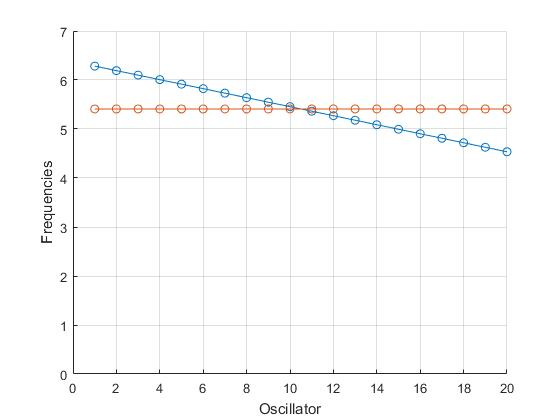
\includegraphics[width=\textwidth]{results/6.b/propaWaveFreq.jpg}
		\caption{}
	\end{subfigure}
	\centering
	\begin{subfigure}[b]{0.49\textwidth}
		\centering
		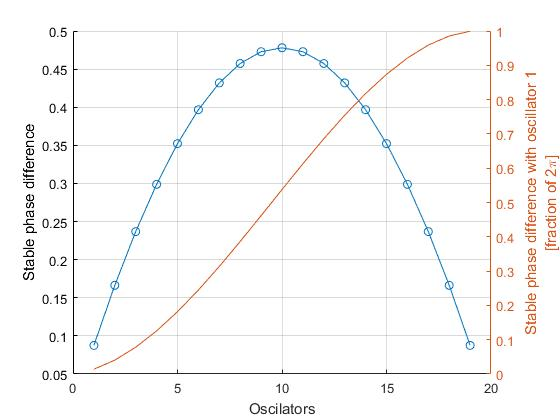
\includegraphics[width=\textwidth]{results/6.b/propaWavePhase.jpg}
		\caption{}
	\end{subfigure}
	\caption{Intrinsic and resulting frequencies for each oscillator (a). Stable phase difference between adjacent oscillator and with first oscillator (b). The simulation was performed with 20 oscillators, a coupling strength of 10 and a linear gradient of intrinsic frequencies with drift -0.092\,rad/step. The simulation parameters fulfil the phase locking condition from the previous section.}\label{prop}
\end{figure}

The linear gradient yields to a quadratic stable phase difference between adjacent oscillators (\ref{prop}). The stable phase difference with oscillator 1 was found using the cumulative sum of the phase differences between adjacent oscillators. The phase difference between the first and last oscillators is approximatively $2\pi$ i.e. their are in phase as sinus function is $2\pi$-periodic. This correspond to a travelling wave with wavelength equal to the length of the lamprey spinal cord.

\begin{figure}[h]
	\centering
	\begin{subfigure}[b]{0.49\textwidth}
		\centering
		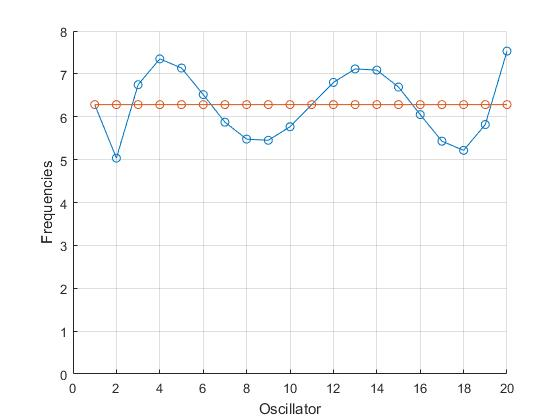
\includegraphics[width=\textwidth]{results/6.b/standWaveFreq.jpg}
		\caption{}
	\end{subfigure}
	\centering
	\begin{subfigure}[b]{0.49\textwidth}
		\centering
		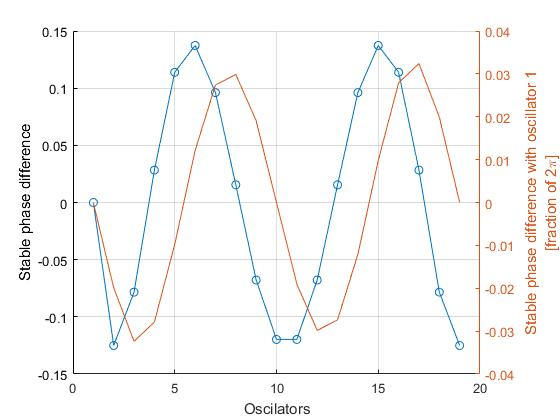
\includegraphics[width=\textwidth]{results/6.b/standWavePhase.jpg}
		\caption{}
	\end{subfigure}
	\caption{Intrinsic and resulting frequencies for each oscillator (a). Stable phase difference between adjacent oscillator and with first oscillator (b). The simulation was performed with 20 oscillators, a coupling strength of 10 and a polynomial gradient of intrinsic frequencies: $\omega_i = \omega_{1} + (-1.95\ 10^{-6}\times(i-1)^7 -1.37\ 10^{-4}\times(i-1)^6) -3.56\ 10^{-6}\times(i-1)^5 +4.12\ 10^{-2}\times(i-1)^4 -1.76\ 10^{-1}\times(i-1)^3 -2.43\ 10^{-1}\times(i-1)^2 +3.16\times(i-1)-4.02$. The simulation parameters fulfil the phase locking condition (i.e. the absolute value of the components of vector S are all inferior or equal to 1).}\label{stand}
\end{figure}

The polynomial gradient yields to a quasi-sinusoidal stable phase difference between adjacent oscillators (\ref{stand}). The stable phase difference with oscillator 1 was found using the cumulative sum of the phase differences between adjacent oscillators. Including the first and last oscillator there are 5 locations where the phase difference with oscillator 1 is null, these points are in phase with each other. This correspond to a standing wave along the lamprey with 5 nodes and therefore 4 anti-nodes.

\begin{figure}[h]
	\centering
	\begin{subfigure}[b]{0.49\textwidth}
		\centering
		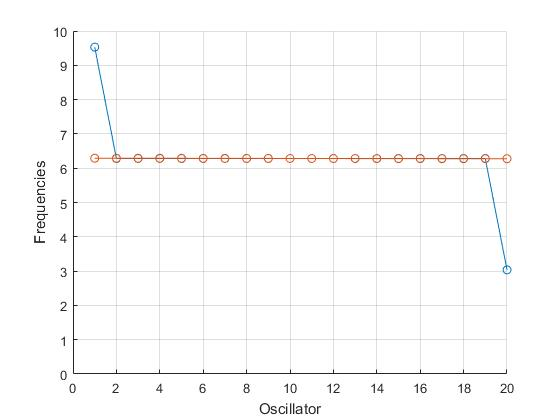
\includegraphics[width=\textwidth]{results/6.b/compSP_DP_CPFreq.jpg}
		\caption{}\label{3a}
	\end{subfigure}
	\centering
	\begin{subfigure}[b]{0.49\textwidth}
		\centering
		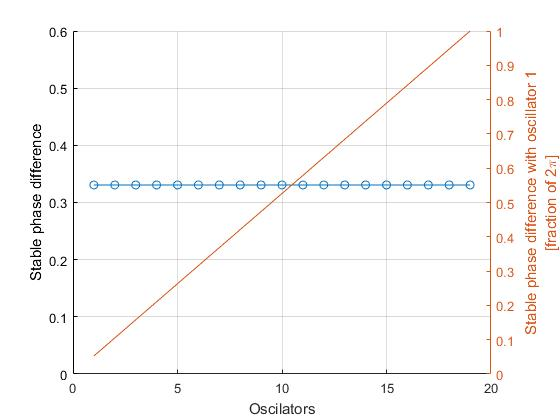
\includegraphics[width=\textwidth]{results/6.b/compSP_DP_CPPhase.jpg}
		\caption{}\label{3b}
	\end{subfigure}
	\centering
	\begin{subfigure}[b]{0.49\textwidth}
		\centering
		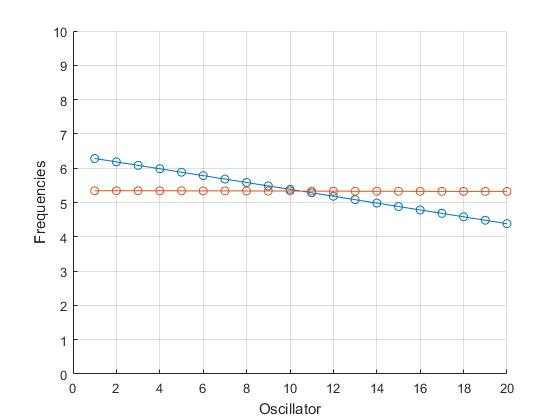
\includegraphics[width=\textwidth]{results/6.b/compSP_DP_DPFreq.jpg}
		\caption{}\label{3c}
	\end{subfigure}
	\centering
	\begin{subfigure}[b]{0.49\textwidth}
		\centering
		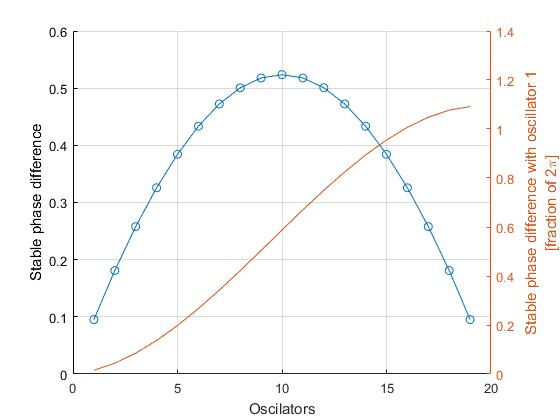
\includegraphics[width=\textwidth]{results/6.b/compSP_DP_DPPhase.jpg}
		\caption{}\label{3d}
	\end{subfigure}
	\begin{subfigure}[b]{\textwidth}
		\centering
		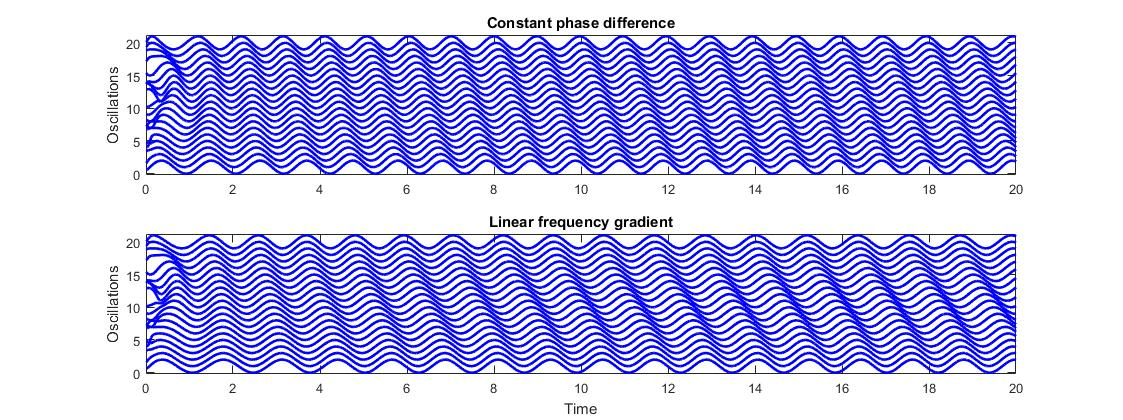
\includegraphics[width=\textwidth]{results/6.b/compSP_DP_oscillations.jpg}
		\caption{}\label{3e}
	\end{subfigure}
	\caption{Intrinsic and resulting frequencies for each oscillator (\ref{3a}-\ref{3c}). Stable phase difference between adjacent oscillator and with first oscillator (\ref{3b}-\ref{3d}). The simulations were performed for non linear gradient (\ref{3a}-\ref{3b}) given by: $\omega_{1} = 2\pi + 3.2469 ,\omega_{20} = 2\pi - 3.2469 , \omega_{i} = 2\pi$ and for a linear gradient (\ref{3c}-\ref{3d}) with drift -0.1\,rad/step. For all the simulations the number of oscillators was 20 and the coupling strength 10 and the same initial conditions. Oscillation as a function of time (\ref{3e}) for both intrinsic frequency models.}
\end{figure}

The linear frequency gradient produces a non constant stable phase difference between  adjacent oscillators which can be seen in figure \ref{3d} and \ref{3e}. The non linear gradient described in the legend produces a constant phase difference between adjacent oscillators which can be seen in figure \ref{3b} and \ref{3e} with straight wavefront.

\subsection{External load (6.c)}
In this part an external load with frequency $\omega_{mech}$ is applied to the tail of the lamprey with a sensory coupling strength $a_{sens}$:
\begin{align*}
\frac{d}{dt}\psi_N &= \omega_N + a \sin(\psi_{N-1}-\psi_N) + a_{sens} \sin(\omega_{mech}.t-\psi_N) \\
\frac{d}{dt}\mathbf{\phi} &= \mathbf{\Omega} + A \mathbf{S} - a_{sens} \sin(\omega_{mech}.t-\psi_N)\ [0, \ldots, 0,\, 1]'
\end{align*}
And therefore in phase locking regime:
\begin{align*}
\frac{d}{dt}\mathbf{\phi} &= 0\\
\mathbf{S} &= A^{-1}(a_{sens}\sin(\omega_{mech}.t-\psi_N)\ [0, \ldots, 0,\, 1]'-\mathbf{\Omega})
\end{align*}
The condition for phase locking is that for every element $s_i$ of $\mathbf{S}$: $|s_i|\leq1$.
Therefore setting the coupling strength to 10 and the frequency drift to -0.1\,rad/step, and as $-1\leq\sin(x)\leq1 \forall x \in \mathbf{R}$, we can calculate a value for the sensor coupling strength such that the condition for phase locking is verified.

We studied the effect of the sensor coupling strength and mechanical excitation frequency on the resulting frequency of the oscillators (\ref{4a}-\ref{4c}) while checking for phase lock conditions (\ref{4b}-\ref{4d}). As expected for the chosen set of parameters the standard deviation of the phase differences between the oscillators is bounded with small periodic perturbation corresponding to small variations of few last oscillators. We can conclude that the system is in a phase locking regime in a less strict sense than in the previous sections.

From the figure \ref{4c} we can see that the effect of sensor coupling affects more the last oscillator and that its resulting frequency converge toward the mechanical excitation's frequency. The frequency of the first oscillator also increases for sensor coupling strength higher that approximatively 1.

From the figure \ref{4a} we can see that there is a range of excitation's frequencies ($0.8\times2\pi-0.95\times2\pi$\,rad/s) for which the last oscillator converges to $\omega_{mech}$ and the frequency of the first oscillator increases steadily. This range is close from the resulting frequency of the oscillator without mechanical excitation which is around $0.85\times2$. For higher excitations frequencies the frequency drops possibly because the intrinsic and excitation oscillations compensates each other. Neither the last nor the first oscillator frequencies converges toward $\omega_{mech}$ at higher mechanical excitation frequencies.
\newpage

\begin{figure}[h]
	\centering
	\begin{subfigure}[b]{0.49\textwidth}
		\centering
		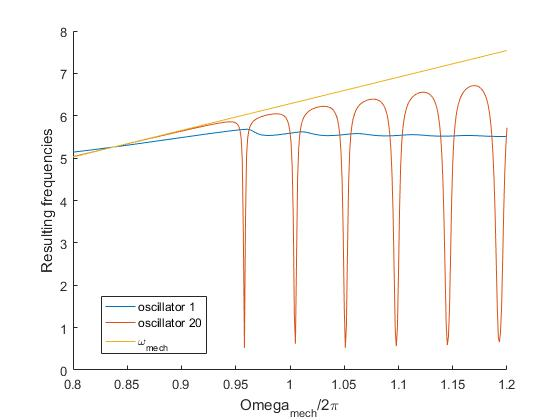
\includegraphics[width=\textwidth]{results/6.c/Freq_A_const.jpg}
		\caption{}\label{4a}
	\end{subfigure}
	\centering
	\begin{subfigure}[b]{0.49\textwidth}
		\centering
		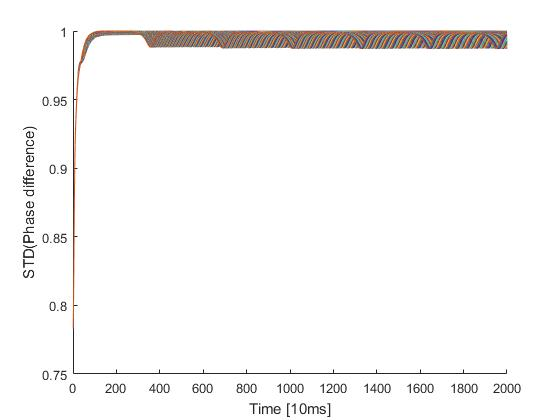
\includegraphics[width=\textwidth]{results/6.c/Phase_A_const.jpg}
		\caption{}\label{4b}
	\end{subfigure}
	\centering
	\begin{subfigure}[b]{0.49\textwidth}
		\centering
		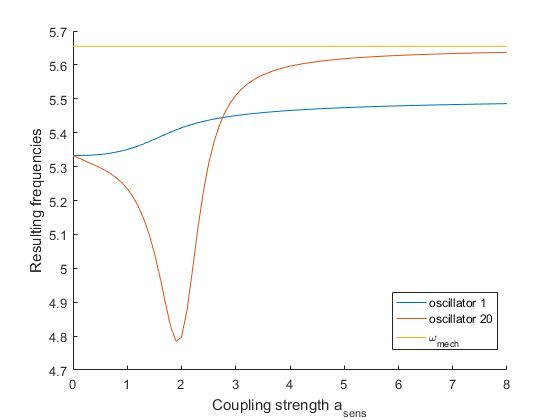
\includegraphics[width=\textwidth]{results/6.c/Freq_O_const.jpg}
		\caption{}\label{4c}
	\end{subfigure}
	\centering
	\begin{subfigure}[b]{0.49\textwidth}
		\centering
		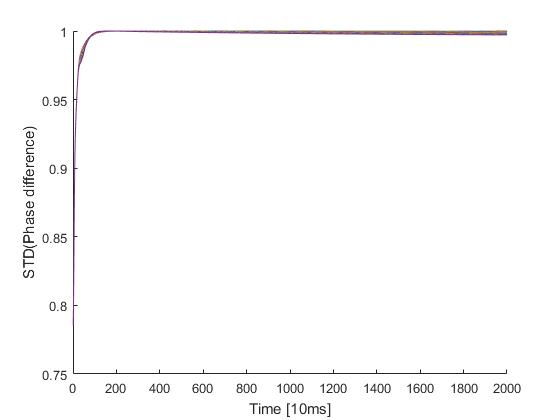
\includegraphics[width=\textwidth]{results/6.c/Phase_O_const.jpg}
		\caption{}\label{4d}
	\end{subfigure}
	\caption{Resulting frequencies of the oscillator 1 and 20 as well as mechanic excitation(\ref{4a}-\ref{4c}). In figure \ref{4a} the coupling strength was kept constant at 8 while the frequency of the mechanic excitation was varied. In figure \ref{4c} the mechanic excitation's frequency was kept constant while the coupling strength was varied. Figures \ref{4b} and \ref{4d} represent the normalized standard deviation of the phase difference between oscillators as a function of time to check for phase locking. All the simulations were done for models with coupling strength of 10, frequency drift of -0.1\,rad/step and 20 oscillators.}
\end{figure}

\FloatBarrier

\section{Comparing neuronal oscillators with phase oscillators}
\subsection{General behaviour (7.a)}

We saw  on the previous section that a phase oscillators with a good coupling has a smouth behaviour, it is also the case for a neuronal oscillator. A practical example could be 2 pendulums with an independant source of excitation coupled with a spring. If they have two intrinsic different frequency at the begining, there will be a transitory phase until they converge to the same freqency with some phase depending on the coupling strengh. The two signals in time look like sinusoidal curves. See figure \ref{2phase}.

\begin{figure}[!h]
	\centering
	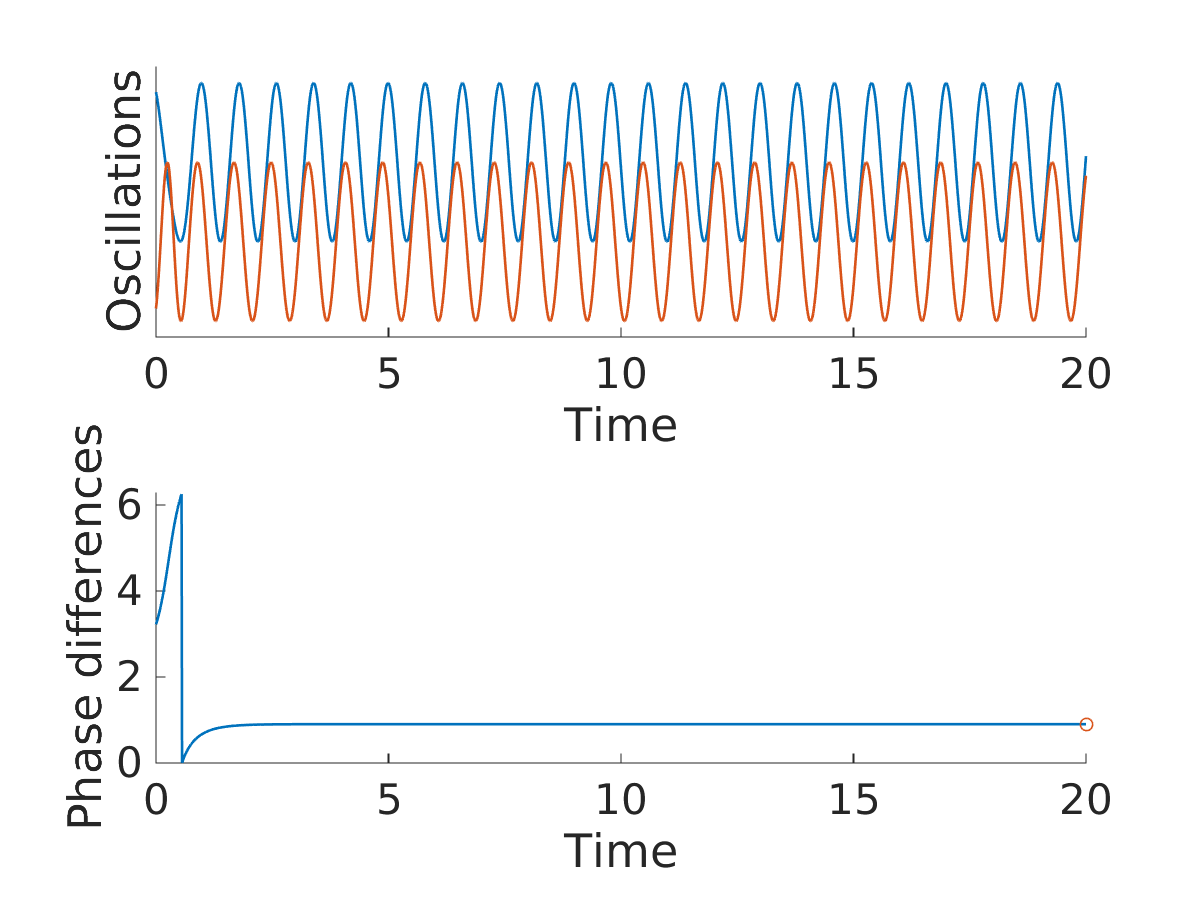
\includegraphics[width=0.5\textwidth]{fig/2phase.png}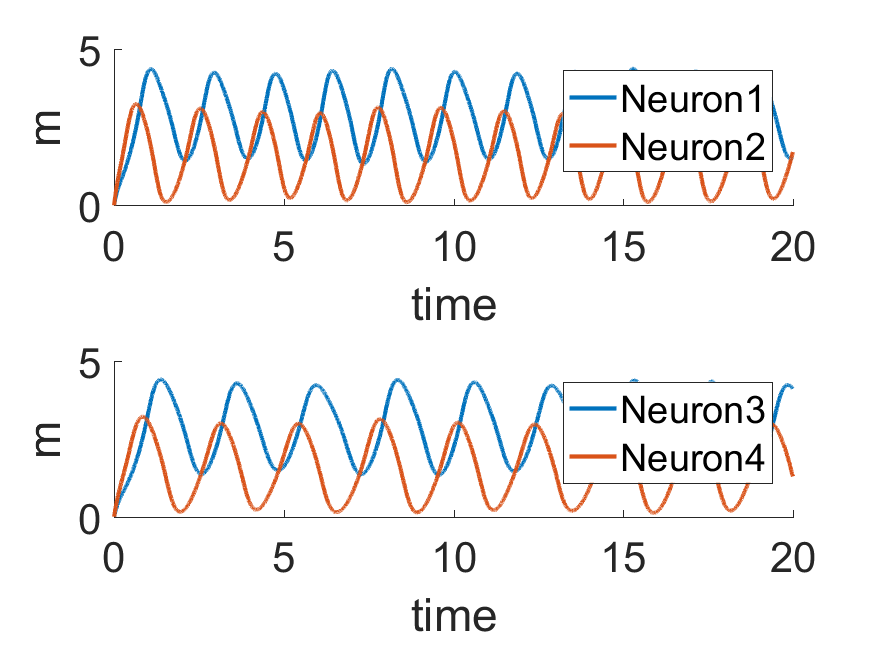
\includegraphics[width=0.5\textwidth]{fig/neuron1}
	\caption{On the left picture, a stable phase oscillator and some crazy stable neuronal oscillations using a strong negative coupling on the right picture.}\label{2phase}
\end{figure}

In opposition a phase oscillator, it is possible for a neuronal oscillator to reach different modes of stable oscillations even with some highly non linear curves using a high negative coupling strengh, see figure \ref{crazy}.

\begin{figure}[!h]
	\centering
	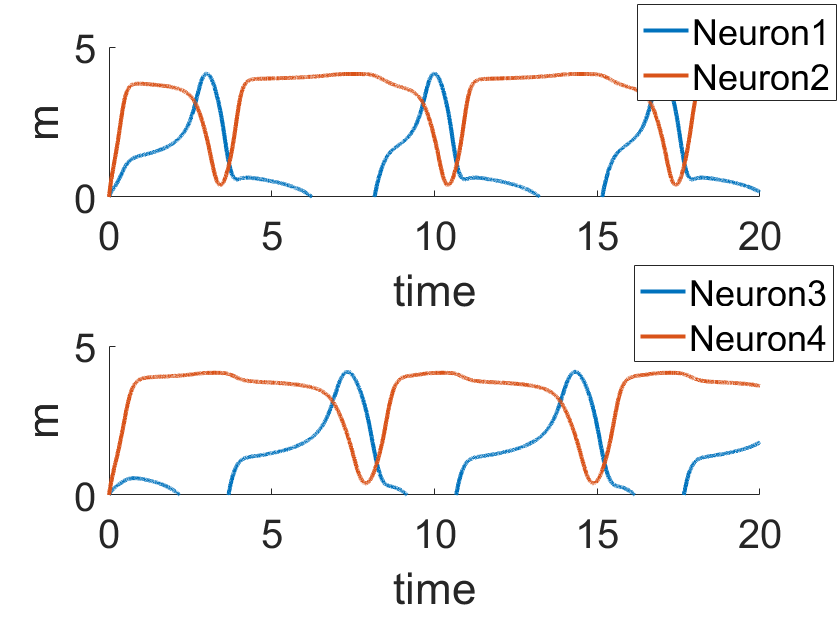
\includegraphics[width=0.5\textwidth]{fig/crazy.png}
	\caption{A stable neuronal oscillations using a strong negative coupling.}\label{crazy}
\end{figure}


When playing with the coupling strengh, one can observe two different behaviours. For the phase oscillators, a high coupling strengh results in the two masses oscillating at the same phase and frequency. If we add a strong positive coupling strengh to two neuronal oscillators, for example neuron 1 and 3, one can observe that the neurons will no longer oscillate but saturate to the maximum value because they excite one the other, see figure \ref{kill}. The neurons 2 and 4 will be killed because of the negative feedback from neurons 1 and 2.

\begin{figure}[!h]
	\centering
	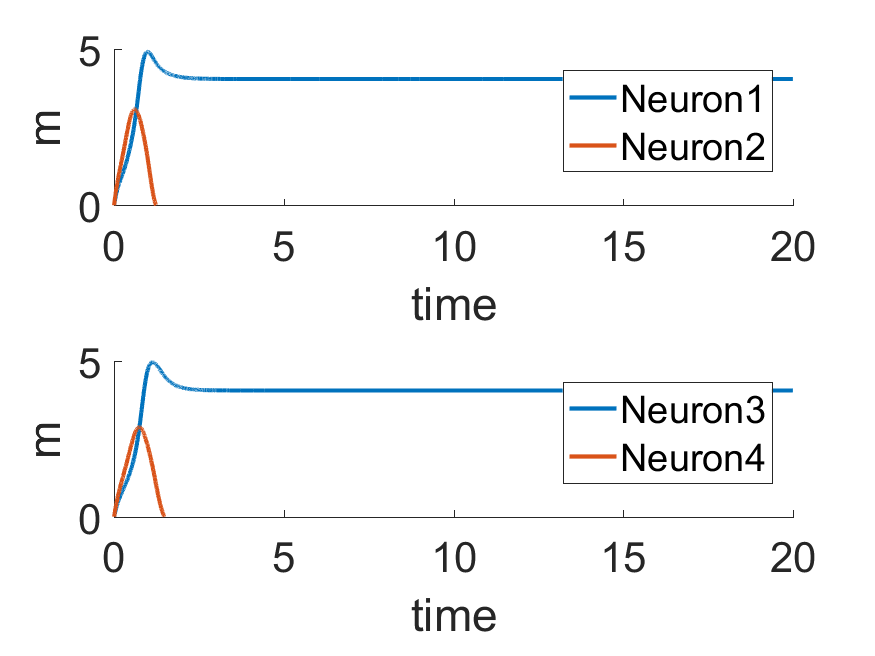
\includegraphics[width=0.5\textwidth]{fig/kill.png}
	\caption{Neurons with a high coupling strengh resulting in no oscillations.}\label{kill}
\end{figure}

\newpage

\subsection{Comparing forced oscillators (7.b)}

If the periodic input is in the same range of frequency as the neuron 1, one can distinguish two extrem cases. Firstly, if the coupling strengh is low, the neuron 3 will lightly feel the influence of the input periodic signal, see fig \ref{7b}.

\begin{figure}[!h]
	\centering
	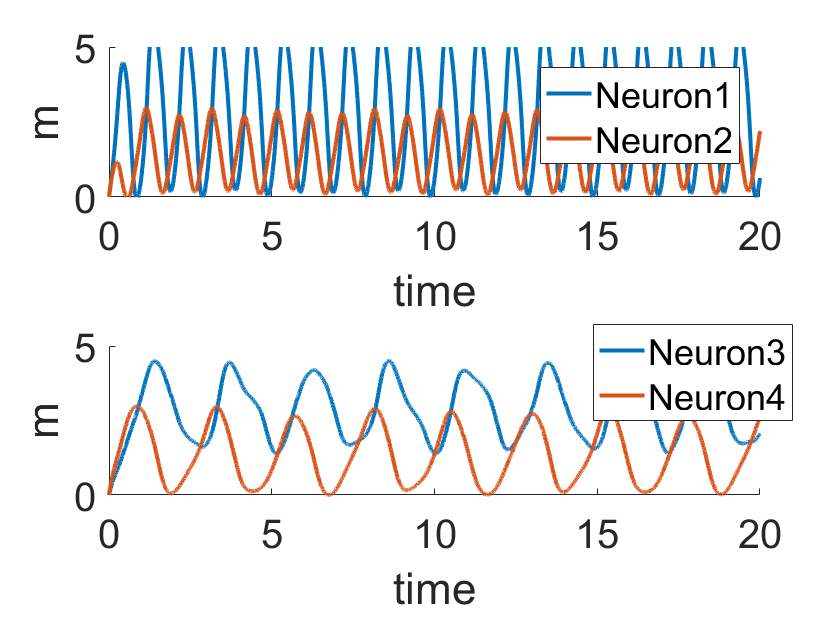
\includegraphics[width=0.5\textwidth]{fig/7b.png}
	\caption{Neuronal oscillators with a low coupling strengh and a periodic input on the first neuron.}\label{7b}
\end{figure}

Secondly, one can observe that even if the neurons are overconstrained and then saturate, there will be a residual oscillations, see fig \ref{sat}. This is interesting because we can imagine that the environement dictate the coupling strengh and our neuronal system could oscillate in different modes depending one the coupling strengh.

\begin{figure}[!h]
	\centering
	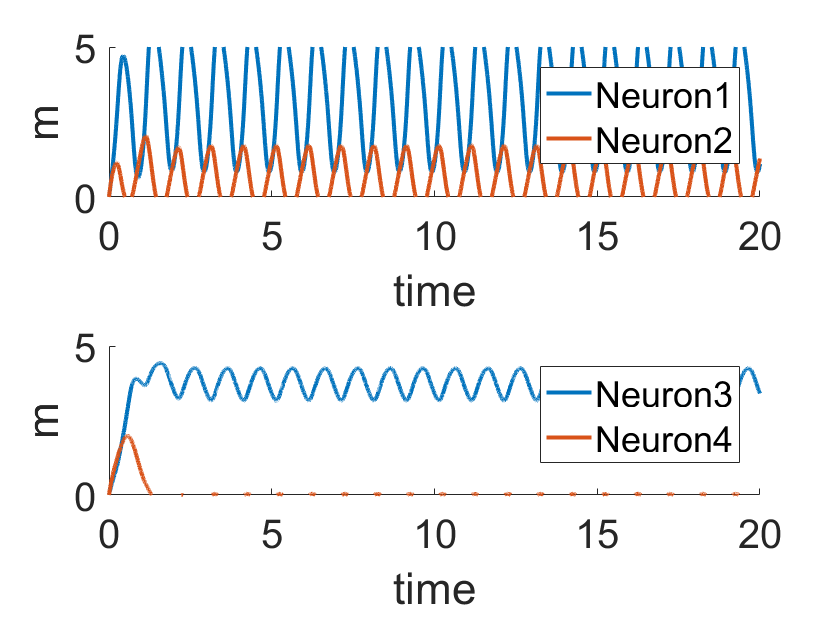
\includegraphics[width=0.5\textwidth]{fig/sat.png}
	\caption{A high positive coupling strengh on a neuronal oscillator excited by a periodic signal on the neuron 1.}\label{sat}
\end{figure}

\newpage

In the case where the frequency of the input signal is way higher than the instrinsic frequency, the transmition of the excitation for a both type of oscillators is low if the coupling strengh isn't too high. If the constrain is too high, the neuronal oscillator saturate as seen in the previous figure and the phase oscillator will have some chaotic behaviour. One can see on figure \ref{dd} that they have same kind of behaviour if one simulate the systems with parameters of the same order.

\begin{figure}[!h]
	\centering
	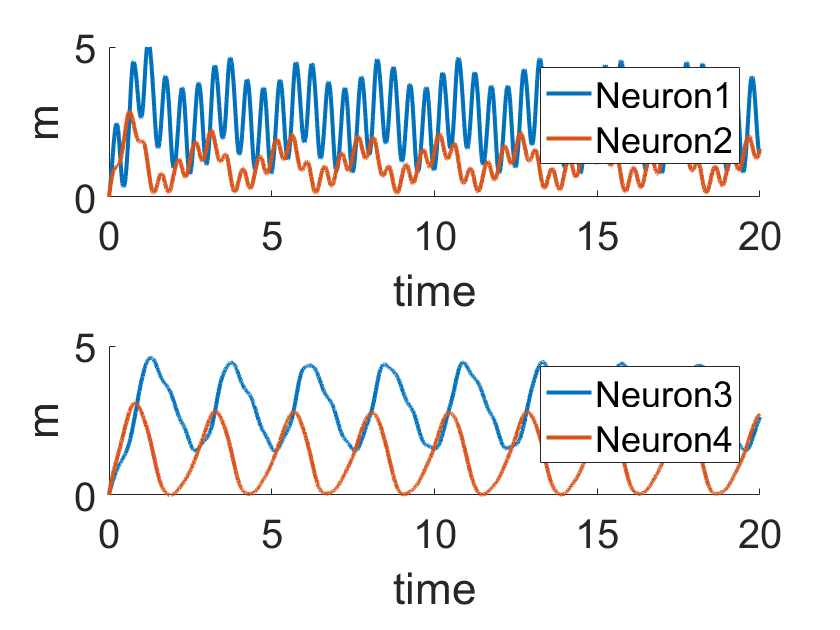
\includegraphics[width=0.5\textwidth]{fig/dd.png}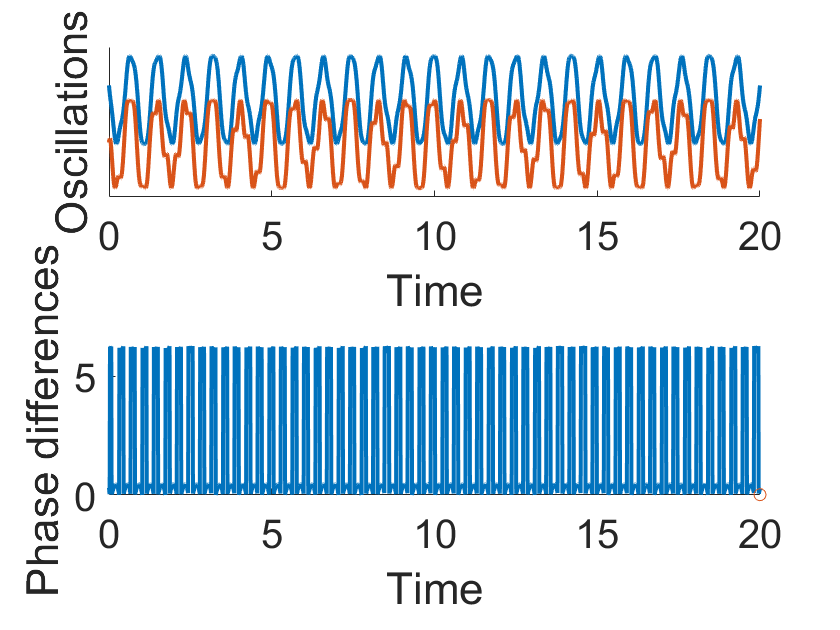
\includegraphics[width=0.5\textwidth]{fig/chao.png}
	\caption{On the left picture, a low constrain neuronal oscillator that doesnt saturate. On the right a chain phase oscillator with the same corresponding coupling strengh. In both case, a periodic input with a frequency 4 time higher than their intrinsic frequency is applied on one side.}\label{dd}
\end{figure}
	
\end{document}
